\section{Casos de uso}
Para ayudarnos a analizar el problema, hemos desarrollado casos concretos de uso de la aplicación.
Al tratarse de un sistema interactivo, es irreal pretender considerar todos los casos de uso.
En los siguientes ejemplos puede haber omisiones.

\subsection{Diagrama de casos de uso}
Este diagrama intenta resumir los posibles casos de uso de la aplicación:\\
{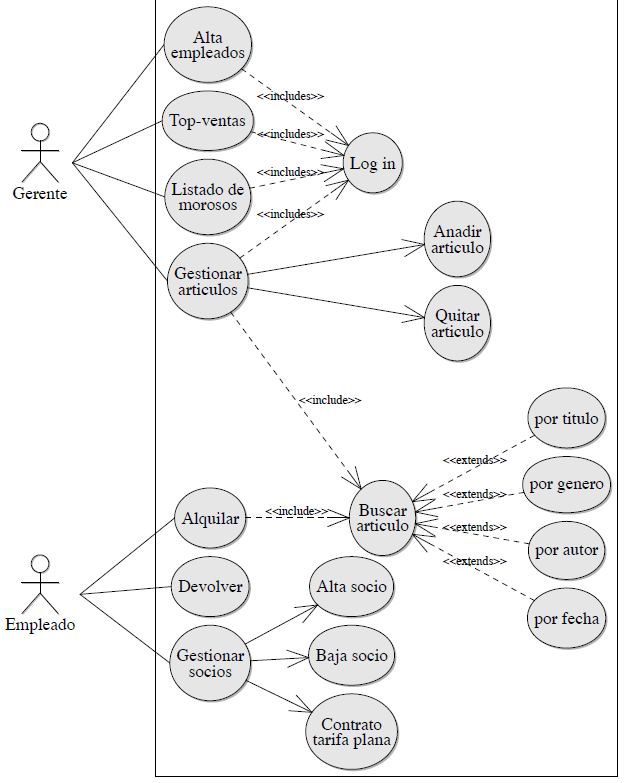
\includegraphics[width=14cm, height=14cm, keepaspectratio]{img/example.png}\\


\subsection{Descripción de casos de uso}
A continuación se detallan tres casos de uso que hemos estimado importantes: un alquiler, una devolución y una acción administrativa. El criterio que hemos seguido es la frecuencia de ocurrencia.
Para simplificar las descripciones y diagramas nos referiremos conjuntamente a películas, series y discos como artículos. Además, consideramos al empleado y socio como una misma entidad ya que los empleados solo actúan como nexo entre el socio y el software. 

\subsubsection{Préstamo}
\begin{description-especial}
	\item[Actor primario]         	\emph{Empleado}, atendiendo a \emph{socio}
	\item[Interesados y objetivos]	El socio desea alquilar un artículo, Smallville por ejemplo. El empleado debe procesar el trámite.
	\item[Precondiciones]         	El socio debe ser un socio registrado por el sistema.
	\item[Garantía de éxito (postcondiciones)] El socio alquila el artículo y el préstamo queda registrado en la aplicación.
	\item[Escenario principal de éxito] Interacciones del escenario, numeradas:
	\begin{enumerate}
		\item El empleado introduce el DNI/NIA del socio.
		\item El empleado busca el artículo solicitado, obteniendo el UID del artículo.
		\item Se verifica que los datos introducidos sean válidos, indicándoselo al empleado.
		\item El socio debe ahora abonar el importe del préstamo: efectivo o tarjeta.
		\item Se guarda un registro de la transacción y se genera la factura.
	\end{enumerate}
	\item[Extensiones (flujos alternativos)] Escenarios excepcionales:
	\begin{itemize}
		\item[3b.] El socio tiene cobros pendiente o artículos pendiente por devolver.
		\begin{enumerate}
			\item[i.]  El sistema no deja alquilar el artículo.
			\item[ii.] El empleado puede cancelar la operación.
		\end{enumerate}

		\item[3c.] El empleado no encuentra el artículo solicitado.
		\begin{enumerate}
			\item[i.] El empleado puede cancelar la operación.
		\end{enumerate}

		\item[4b.] El socio, por el motivo que alegue, desea cancelar la operación (no tiene dinero por ejemplo.)
		\begin{enumerate}
			\item[i.] El empleado puede cancelar la operación.
		\end{enumerate}
	\end{itemize}

	\item[Requisitos especiales] Tiempo de respuesta en la búsqueda de artículos moderadamente rápido.
	\item[Lista de variaciones de tecnología y datos] Ninguno
	\item[Frecuencia de ocurrencia] Entre 10 y 100 (depende del éxito del videoclub).
\end{description-especial}

\subsubsection{Devolución}
\begin{description-especial}
	\item[Actor primario]         	\emph{Empleado}, atendiendo a \emph{socio}
	\item[Interesados y objetivos]	Se desea devolver un artículo alquilado (volumen SmallVile)
	\item[Precondiciones]         	El socio debe ser un socio registrado por el sistema.
	\item[Garantía de éxito (postcondiciones)] El socio devuelve el artículo, Smallville, y el sistema detecta la devolución.
	\item[Escenario principal de éxito] Interacciones del escenario, numeradas:
	\begin{enumerate}
		\item El empleado introduce el DNI/NIA del socio y el UID del artículo.
		\item Se verifica que los datos introducidos sean válidos.
		\item El sistema se actualiza, marcando el artículo como disponible, e indicando que el socio ya no lo tiene.
	\end{enumerate}
	\item[Extensiones (flujos alternativos)] Escenarios excepcionales:
	\begin{itemize}
		\item[2b.] El socio ha devuelto el artículo fuera del período asignado.
		\begin{enumerate}
			\item[i.]  El sistema indica la cantidad a abonar. Si el socio no dispone del dinero solicitado, puede cancelar la operación pero seguirá teniendo la sanción y el artículo.
			\item[ii.] Si paga, el préstamo se devuelve y el sistema se actualiza.
		\end{enumerate}
	\end{itemize}

	\item[Requisitos especiales] Ninguno
	\item[Lista de variaciones de tecnología y datos] Ninguno
	\item[Frecuencia de ocurrencia] Entre 10 y 100 (depende del éxito del videoclub).
\end{description-especial}

\subsubsection{Registrar un socio nuevo}
\begin{description-especial}
	\item[Actor primario]                     	Empleado, Socio
	\item[Interesados y objetivos]            	Un individuo desea asociarse al videoclub
	\item[Precondiciones]                     	El cliente no debe estar registrado.
	\item[Garantía de éxito (postcondiciones)]	El cliente queda registrado como socio.
	\item[Escenario principal de éxito]       	Interacciones del escenario, numeradas:
	\begin{enumerate}
		\item El empleado introduce los datos del cliente.
		\item Se verifica que los datos introducidos sean validos.
		\item Los datos quedan guardados en la base de datos.
	\end{enumerate}
	\item[Extensiones (flujos alternativos)] Escenarios excepcionales:
	\begin{itemize}
		\item[2b.] El usuario ya está registrado.
		\begin{enumerate}
			\item[i.]  Se permite la posibilidad de cambiar los datos, o cancelar la operación.
		\end{enumerate}
	\end{itemize}

	Si el usuario ya esta registrado o los datos no son validos, el sistema notificara al empleado.
	\item[Requisitos especiales]                     	Ninguno.
	\item[Lista de variaciones de tecnología y datos]	Ninguno.
	\item[Frecuencia de ocurrencia] Entre 1 y 10 (depende del éxito del videoclub).
\end{description-especial}